Single high-order elements can represent an equivalent number of degrees of freedom.
This approach has been investigated for solid mechanics problems, such as in \cite{pavarino2010bddc}; although, this work incorporated additional primal degrees of freedom from average values across subdomain edges and faces.

\begin{table}[ht!]
\begin{center}
\begin{tabular}{l ccc ccc}
  \toprule
  $p$  &  \multicolumn{3}{c}{Lumped BDDC}  &  \multicolumn{3}{c}{Dirichlet BDDC}  \\
  %\cmidrule(lr){2-3} \cmidrule(lr){4-5} \cmidrule(lr){6-7}
                      &  $\lambda_{\text{min}}$  &  $\lambda_{\text{max}}$  &  $\kappa$ & $\lambda_{\text{min}}$  &  $\lambda_{\text{max}}$ & $\kappa$  \\
  \toprule
  $p = 2$   &  1.000  &    2.800  &    2.800  &  1.000  &  2.042  &  2.042  \\
  $p = 4$   &  1.000  &   12.948  &   12.948  &  1.000  &  3.242  &  3.242  \\
  $p = 8$   &  1.000  &   59.563  &   59.563  &  1.000  &  5.197  &  5.197  \\
  $p = 16$  &  1.000  &  289.678  &  289.678  &  1.000  &  7.761  &  7.761  \\
  \bottomrule
\end{tabular}
\end{center}
\caption{Condition numbers and maximal eigenvalues for single high-order element subdomains}
\label{table:high_order_element_bddc}
\end{table}

Table \ref{table:high_order_element_bddc} shows the maximal eigenvalues and condition numbers for the symbol of the BDDC preconditioned operator $\tilde{\mathbf{M}}^{-1}_i \left( \boldsymbol{\theta} \right) \tilde{{\color{burgundy}\mathbf{A}}} \left( \boldsymbol{\theta} \right)$ for the two dimensional Poisson problem on single high-order element subdomains with varying polynomial orders.

The improved condition number, and therefore convergence, of the Dirichlet BDDC compared to the lumped BDDC is more significant for high-order elements.
With single high-order element subdomains, the Fast Diagonalization Method approximate inverse subdomain solver can be used for both the subdomain subassembled inverse and subdomain interior inverse, which eliminates the advantage in reduced setup costs for lumped BDDC.

\begin{figure}[!ht]
  \centering
  \subfloat[Lumped BDDC]{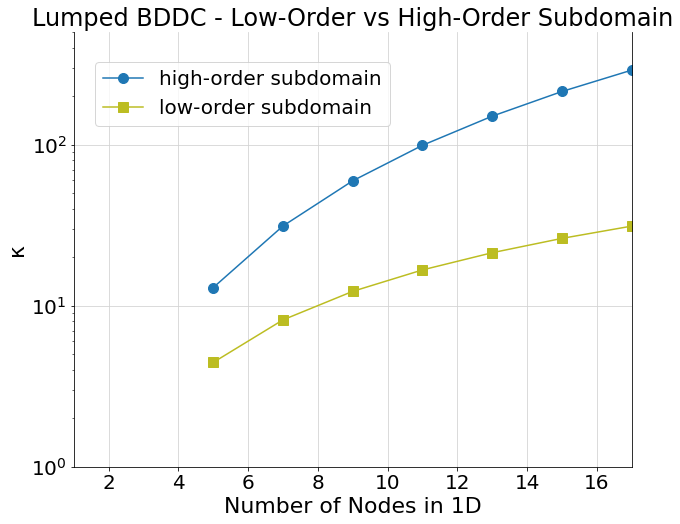
\includegraphics[width=0.48\textwidth]{../img/lowVsHighLumped}\label{fig:lumped_bddc_comparison}}
  \hfill
  \subfloat[Dirichlet BDDC]{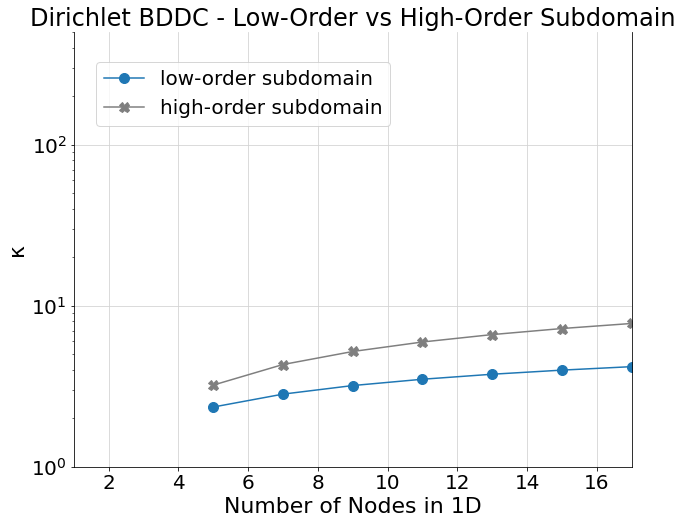
\includegraphics[width=0.48\textwidth]{../img/lowVsHighDirichlet}\label{fig:dirichlet_bddc_comparison}}
  \caption{Low-Order and High-Order Subdomain Condition Number Comparison}
\end{figure}

In Figure \ref{fig:lumped_bddc_comparison} we compare the growth of the condition number for the lumped BDDC preconditioned operator for a subdomain consisting of several linear elements and a subdomain consisting of a single high-order element for the two dimensional Poisson problem.
The condition number grows much more rapidly for a high-order subdomain with an equivalent number of degrees of freedom.

In Figure \ref{fig:dirichlet_bddc_comparison} we compare the growth of the condition number for the Dirichlet BDDC preconditioned operator for a subdomain consisting of several linear elements and a subdomain consisting of a single high-order element for the two dimensional Poisson problem.
In contrast with Figure \ref{fig:lumped_bddc_comparison}, we see that the condition number of the preconditioned operator on the high-order subdomain grows only slighty faster than the condition number of the low-order subdomain.
